\section{Prototype}
\label{sec:prototype}
Here, we discuss our current prototype, challenges, and target applications.
Currently we compile a single shared object (\{envoy,service\}.so) for each side using compiler flags.
It is imperative we intercept syscalls on each side, and as such we must know which side of communication the library is running on to determine which network calls to intercept.
Our library is written in C and is approximately 800 LOC.

\subsection{\sysname Buffer}
Our implementation of \sysname uses \textit{shm\_open} and \textit{mmap} to map shared buffers across the two processes.
The buffer structs container a data buffer, head/tail integers, and pthread mutexes and conditional variables for synchronizing access.
We implemented write/read, and write(v)/read(v) APIs for the buffers since Envoy uses iovec structures for reading and writing.

% Used by prototype
%\begin{table}[!ht]
%    \begin{center}
%        \resizebox{0.5\columnwidth}{!}{
%            \begin{tabular}{ |c|c|c|}
%                \hline
%                \textbf{Function} & \textbf{Envoy} & \textbf{Service} \\
%                \hline \hline
%                socket & X & X \\ \hline
%                connect & X &  \\ \hline
%                listen &  & X \\ \hline
%                accept &  & X \\ \hline
%                poll &  & X \\ \hline
%                select &  & X \\ \hline
%                send &  & X \\ \hline
%                sendto &  & X \\ \hline
%                sendfile &  & X \\ \hline
%                write & X & X \\ \hline
%                read & X & X \\ \hline
%                writev & X &  \\ \hline
%                readv & X &  \\ \hline
%            \end{tabular}
%        }
%        \caption{Library Functions Linked (HTTP/Flask only)}
%        \label{t:libraries}
%    \end{center}
%\end{table}

\begin{table}[!ht]
    \begin{center}
        \resizebox{0.5\columnwidth}{!}{
            \begin{tabular}{ |c|c|c|}
                \hline
                \textbf{Function} & \textbf{Envoy} & \textbf{Service} \\
                \hline \hline
                connect & X &  \\ \hline
                accept &  & X \\ \hline
                write & X & X \\ \hline
                read & X & X \\ \hline
                writev & X &  \\ \hline
                readv & X &  \\ \hline
            \end{tabular}
        }
        \caption{Libc Functions Preloaded (Tiny C Webserver)}
        \label{t:libraries_cserver}
    \end{center}
\end{table}

\subsection{\sysname Network Calls}
The most challenging aspect of \sysname's design is properly intercepting and replicating the behavior of network system calls.
This aspect is especially challenging because Envoy uses unique handlers for request types (UDP, TCP, HTTP\{1,2,3\}, gRPC, Quic).
Further, the service itself may use the network stack in obtuse ways.
%Our investigation of Flask~\cite{flask} has revealed a number of idiosyncrasies with how Flask uses the network stack.
To make \sysname generalizable, one would truly have to intercept every network call (or possible network related).
This task is enormous.
Take for example, how services often tack advantage of configurable aspects of the network stack like \textit{setsockopt}.
Setting options on a particular socket changes the behavior of accept, i/o, and more.
Thus, for \sysname to properly mirror the POSIX API to services in an agnostic way, it would have to model the entire state diagram for sockets.
\todo{Here on}
For our prototype we have focused on HTTP.
In Table-\ref{t:libraries}, we show the calls on each side we intend to link to use \sysname for flask.
Currently our prototype is geared for the tiny C server (Table-\ref{t:libraries_cserver}).

\subsection{Inter-Process Communication}
The implementation started with named pipe as the main Inter-Process Communication (IPC) mechanism. However, due to its unidirectional nature and difficulty in incorporating synchronization mechanisms, we decided the named pipes will not suffice.

As a solution, we used \texttt{shm\_open(2)} to open a file descriptor associated with a region of shared memory and map it to the process using the \texttt{mmap} syscall. We allocate a circular buffer of size $2^{24}$ bytes in this shared region and read and write from it directly using \texttt{memcpy}. We will discuss our choice of the buffer size and how it affects the performance in later section. We allocate two such buffers to provide communication in each direction.

\subsection{Concurrency Problems}
The Envoy process will write the outer request to the buffer and read the service response from the buffer; the service process will read the request (passed on by Envoy) and write the response, as returned by the service. We now have a classic producer-consumer problem.

Our first attempt at the solution was semaphore. We allocated two sempahores, each associated with one buffer, for the purpose of waiting and notifying. However, semaphores did not provide a convenient way to guarantee exclusive access to the buffer. This allowed for data races and caused the program to malfunction.

As an improvement, we moved to using mutexes across processes. Each buffer has a mutex associated with it and also a condition variable. We use these two constructs to guarantee mutual exclusion and to solve the consumer-producer problem.

\subsection{\sysname Status}
We have found tracing the call paths and stack for the networking calls of the C web server and flask tremendously difficult.
As of now we do not have a functional prototype for results.
% TODO: We shoud update this for sure...

\begin{figure*}[!htb]
    \begin{minipage}{0.5\textwidth}
        \centering
        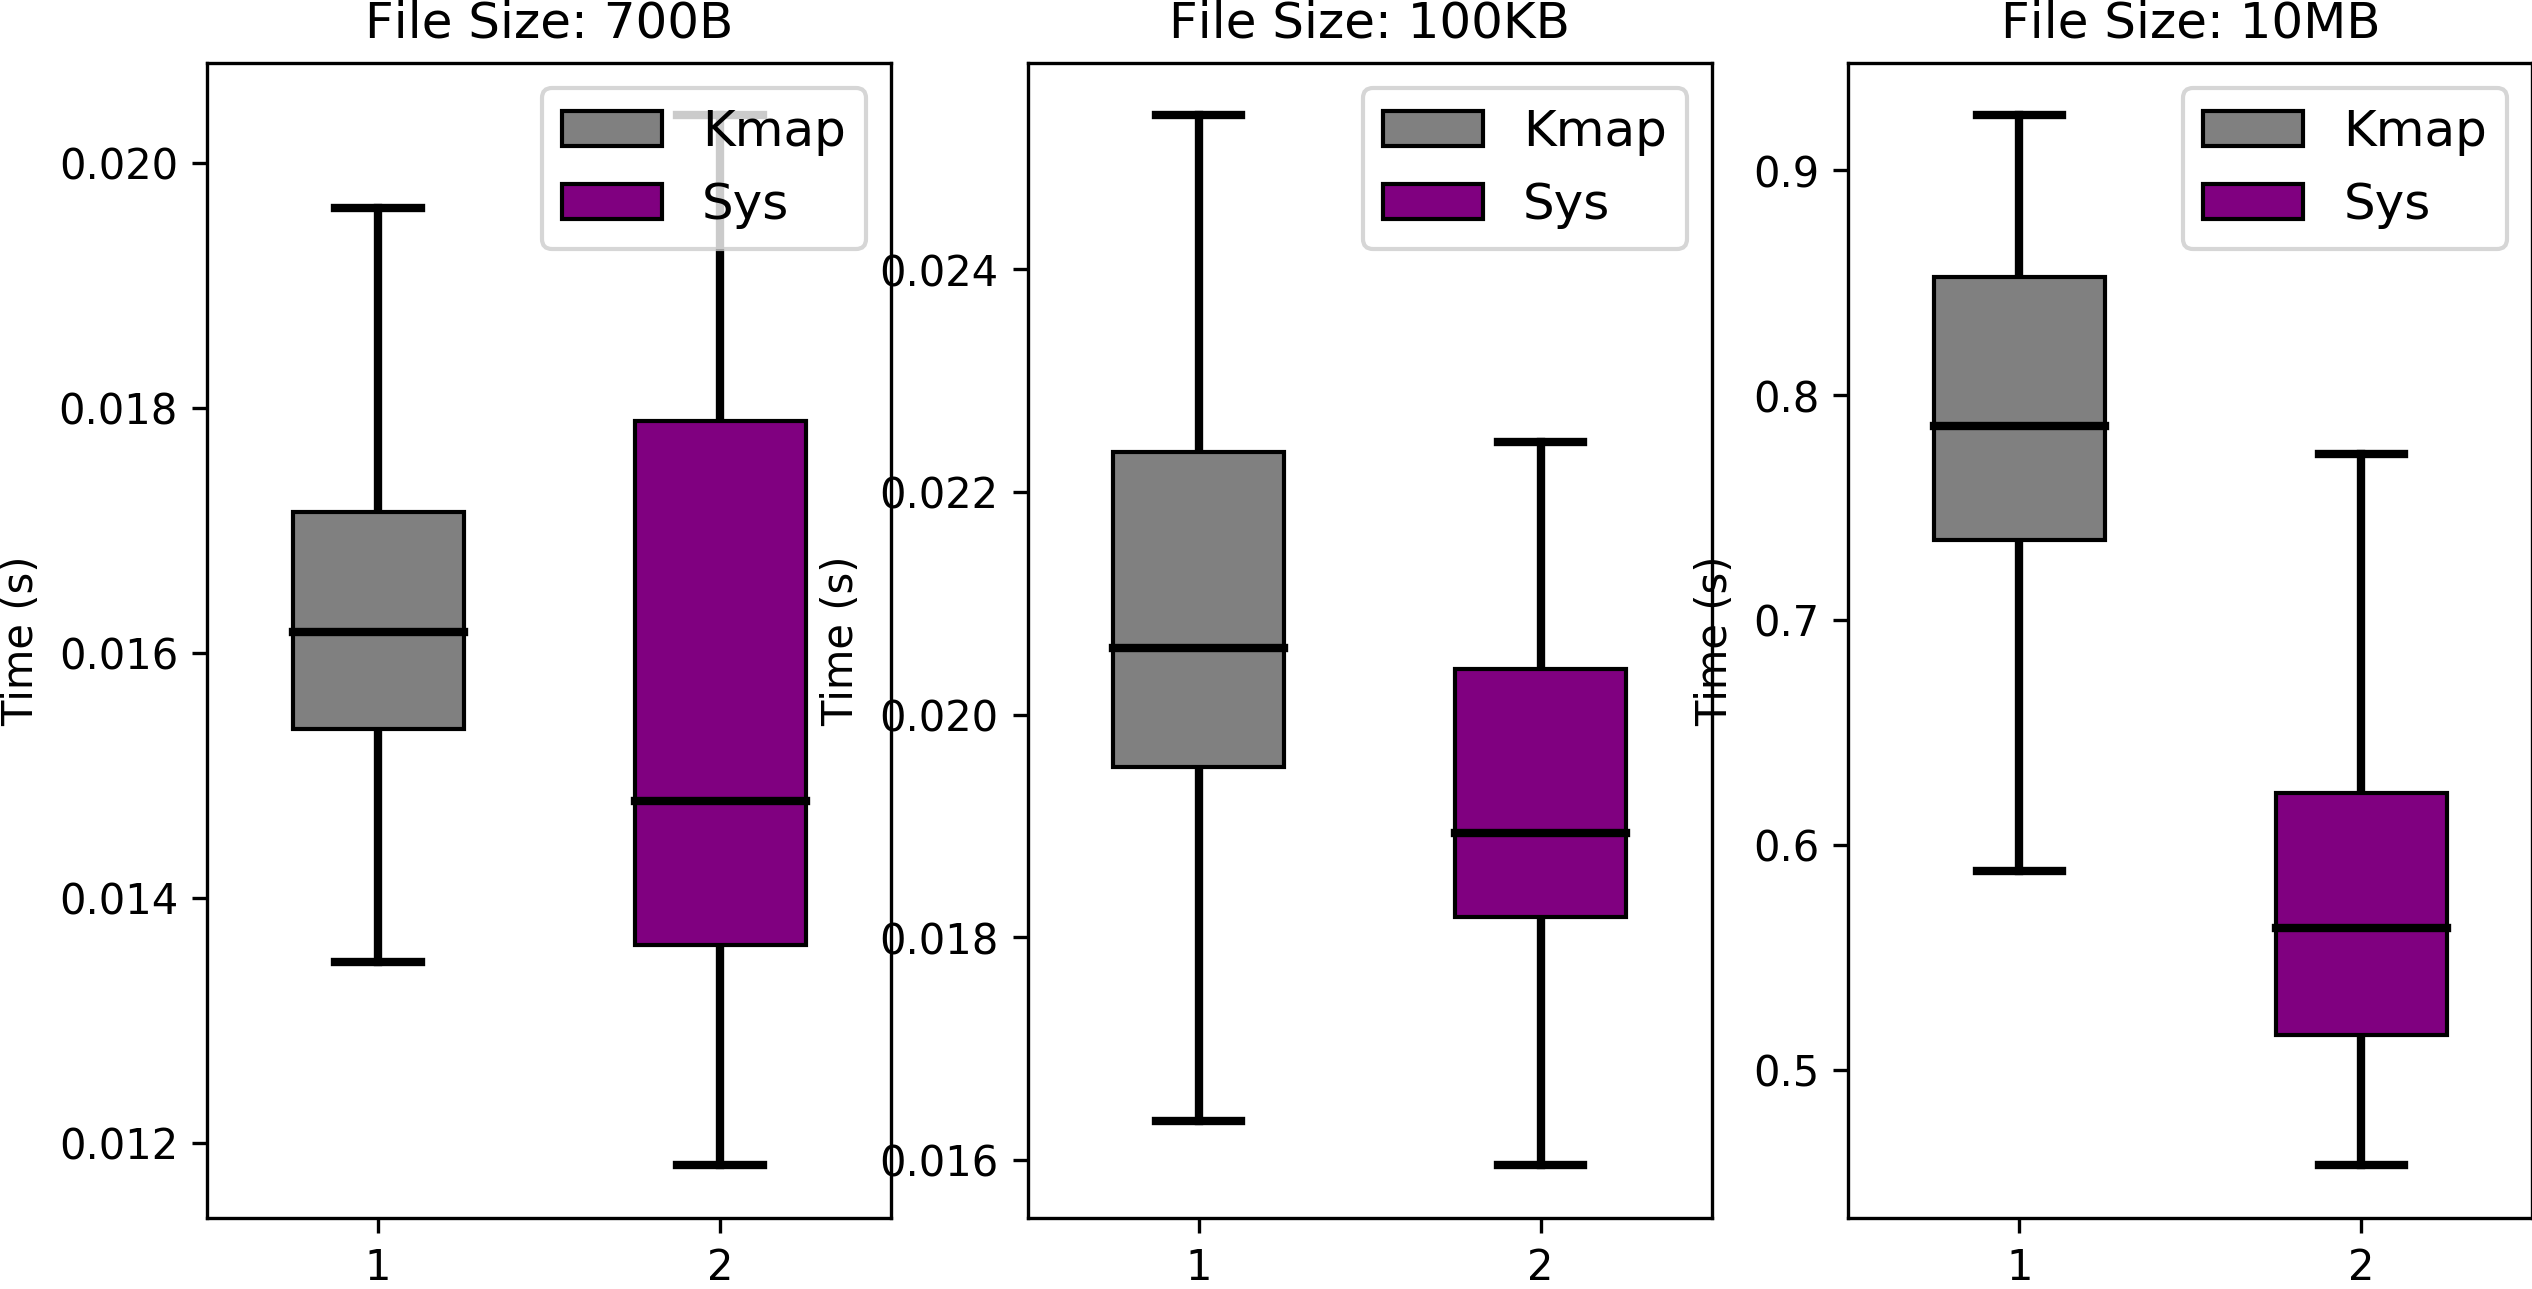
\includegraphics[keepaspectratio=true,width=3in]{figures/evaluation/results.png}
        \caption{Time to Transfer}
        \label{fig:results}
    \end{minipage}%
    \begin{minipage}{0.5\textwidth}
        \centering
        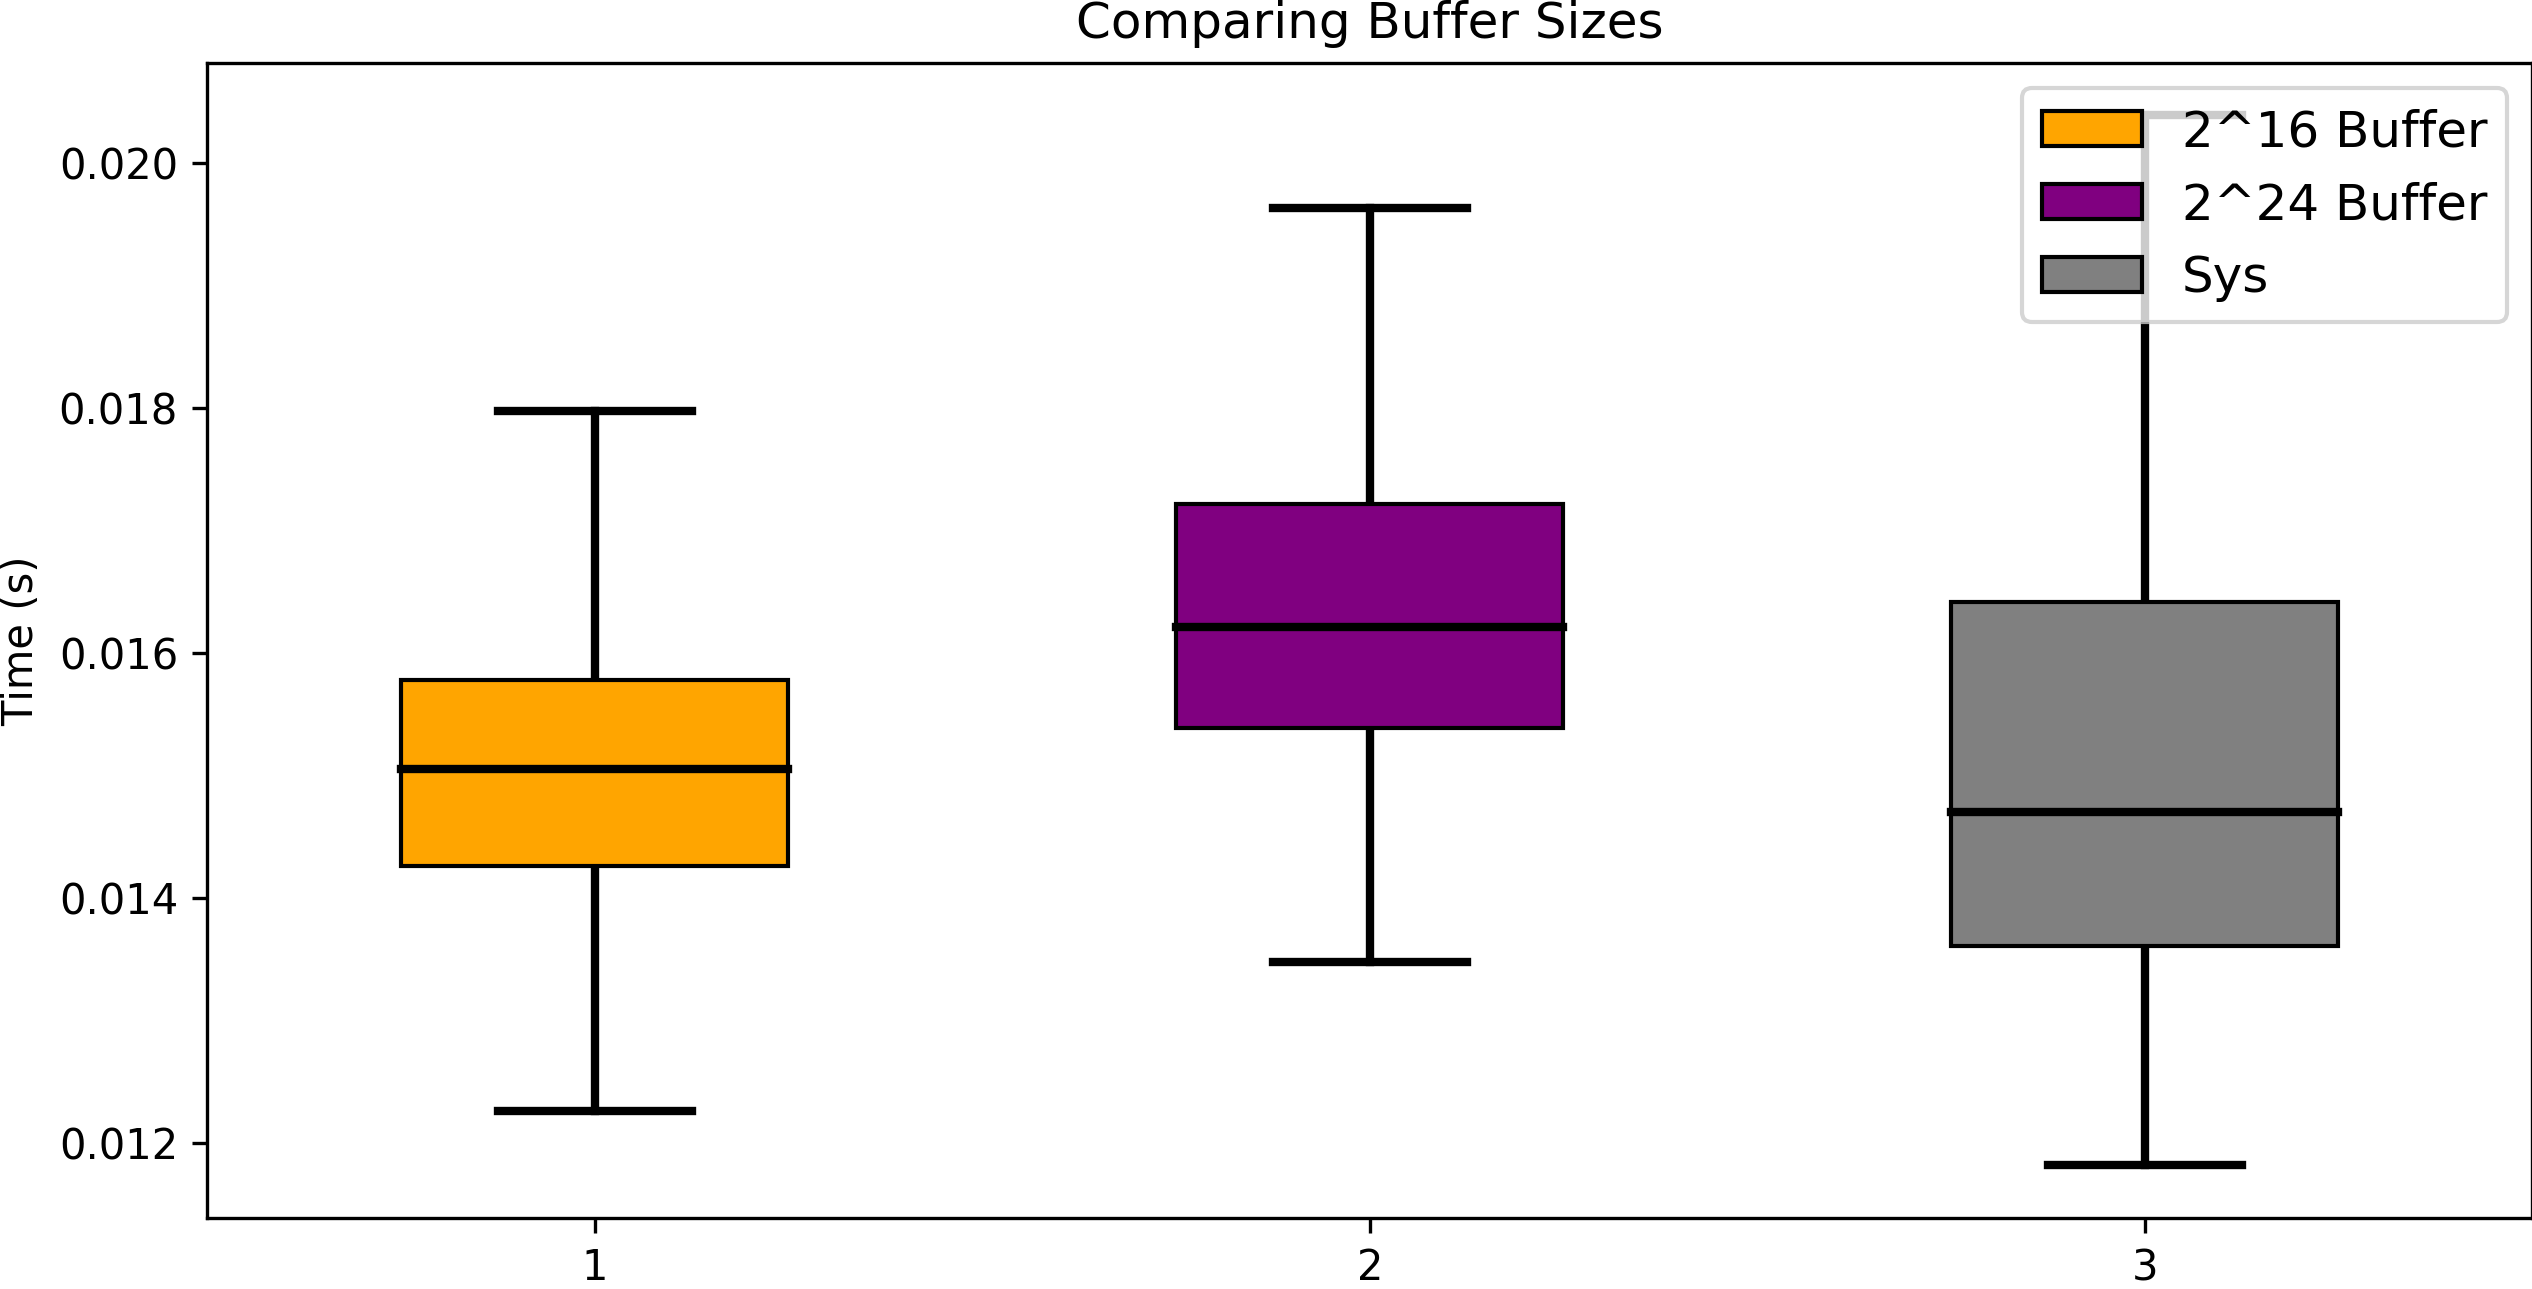
\includegraphics[keepaspectratio=true,width=3in]{figures/evaluation/buf_compare.png}
        \caption{Comparing \sysname Buffer Sizes}
        \label{fig:buf}
    \end{minipage}%
\end{figure*}